
\documentclass[a4paper,oneside, 12pt]{article}
\usepackage{tikz}
\usetikzlibrary{automata, positioning, arrows}
\tikzset{
->,
>=stealth',
node distance=3cm, % specifies the minimum distance between two nodes. Change if necessary.
every state/.style={thick, fill=gray!10}, % sets the properties for each ’state’ node
initial text=$ $, % sets the text that appears on the start arrow
}
\begin{document}
\begin{figure}[ht]
\centering
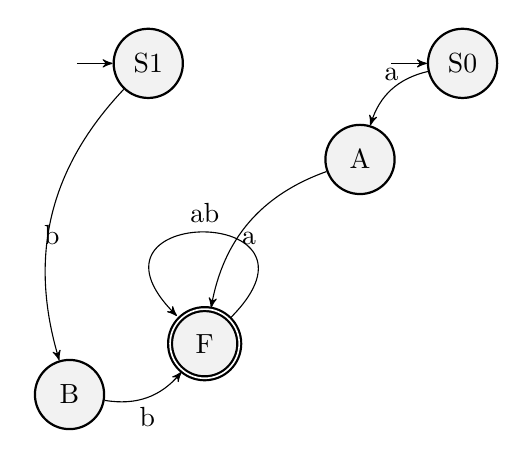
\begin{tikzpicture}
\node[state, initial] at (6.9917, 2.2129) (S0) {S0};
\node[state, initial] at (3, 2.2129) (S1) {S1};
\node[state] at (2.0, -1.9927) (B) {B};
\node[state] at (5.6892, 0.9927) (A) {A};
\node[state, accepting] at (3.7161, -1.3471) (F) {F};
\draw (S0) edge[bend right, above] node {a} (A);
\draw (A) edge[bend right, below] node {a} (F);
\draw (S1) edge[bend right, below] node {b} (B);
\draw (B) edge[bend right, below] node {b} (F);
\draw (F) edge[loop, above] node {ab} (F);

\end{tikzpicture}
%\caption{Caption of the FSM}
%\label{fig:my_label}
\end{figure}
\end{document}
